\chapter{Advisory Intelligence Methods and Limitations}
\label{chap:ai-methods}

\section{Safety Boundary}

The intelligence features help users find suitable items and interpret the information available to them. Their value depends both on how the software handles a request and on whether the underlying data supports the advice. This chapter explains those questions separately: it describes the implemented inputs and outputs, then sets out what remains unverified.

CampusLoop treats every intelligence result as advisory. Search ranks visible products; wanted matching proposes candidates; price advice provides a non-binding interval or an unavailable result; trust summarizes completed-review evidence; and risk clues summarize limited observable activity for an administrator. None of these paths may accept an offer, change an order, hide a listing, disable an account, or resolve a report. Figure~\ref{fig:ai-fallback} shows where the system validates inputs, calls services, falls back, and requires human review.

\begin{figure}[htbp]
  \centering
  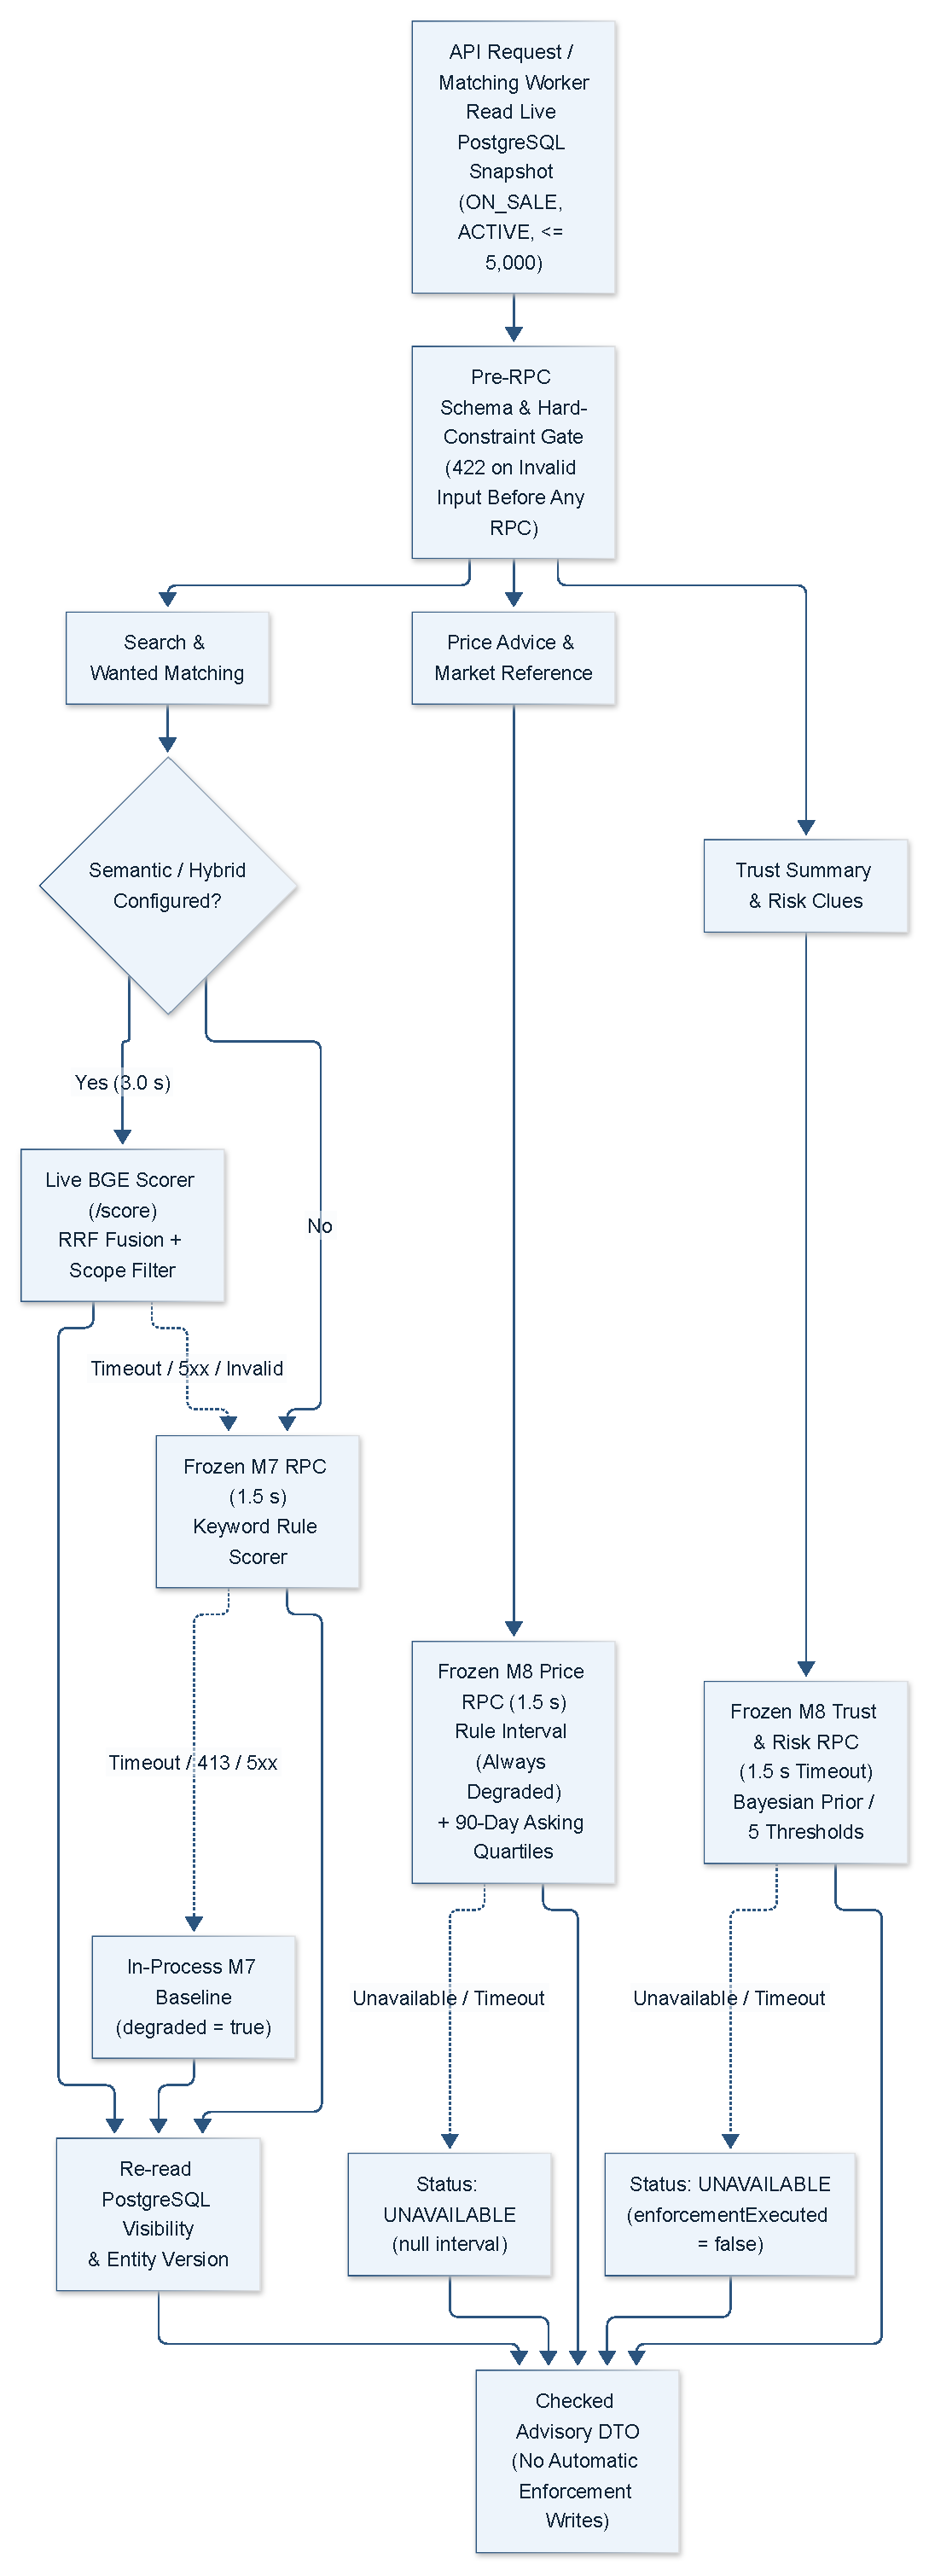
\includegraphics[width=0.92\textwidth]{figures/design/ai-fallback.pdf}
  \caption{Advisory validation, bounded RPC, explicit degradation, and human review.}
  \label{fig:ai-fallback}
\end{figure}

\section{Search and Wanted Matching}

\subsection{Inputs and Output Contract}

Search and wanted matching start from the same eligible catalog. The API takes a snapshot of at most 5,000 products that have not been deleted, are \texttt{ON\_SALE}, and belong to active users. Each candidate contains its stable product and owner identifier, title, description, normalized category and condition, price in fen, campus location, visibility, status, entity version, and publication timestamps.

The request then adds the information needed for the particular task. Search uses the query text, optional category, condition and price filters, mode, and sort order. Wanted matching also uses the wanted-post owner, status, expiry, budget bounds, minimum condition, and required location. These constraints matter because a textually similar product may still be unsuitable for the student's budget or location.

The frozen ranking contract returns product identifiers and versions, a bounded relevance score, deterministic reasons and explanation details, and metadata containing schema, algorithm, dictionary, mode, degradation, and fallback reason. Before exposing results, the API re-reads each ranked product and its owner from PostgreSQL and rejects entries that are no longer public or whose version has changed. A SHA-256 result version covers the stable input snapshot, request, algorithm, options, and requested search mode.

\subsection{Method and Degradation}

Keyword search and wanted matching use the checked-in M7 rule baseline. Optional semantic or hybrid search calls a live semantic service; an unavailable or malformed semantic response is refined by the local catalog-search implementation and marked \texttt{degraded=true} with \texttt{SEMANTIC\_UNAVAILABLE}. The RPC adapter independently computes the frozen rule baseline before accepting a remote result. The adapter checks the response schema and algorithm metadata. It also checks product eligibility, duplicate identifiers, entity versions, score bounds, and exact agreement with the frozen rule explanations. All checks must pass before the response is accepted. Transport failure, timeout, service disablement, or invalid output therefore cannot introduce an unknown candidate.

These checks show whether a response follows the contract. They do not show that its ranking is better. The available evaluation material does not yet include an independently reviewed, representative query set showing an improvement over the original search. Reported ranking quality must therefore be limited to reproducible test outcomes; no production-quality or accuracy claim is made here.

\section{Price Advice}

Price advice receives category, condition, optional original price, title, and description. The current adapter normalizes category and condition, converts original price to fen, and supplies explicit unknown values for purchase age, accessory state, and defect tags. Title and description are not features of the frozen price rule. Title is separately used as a literal keyword for the market-reference query. The frozen M8 service returns a CNY interval, status, explanatory factors, sample size, algorithm version, degradation reason, and disclaimer.

The API accepts the price response only when it follows the frozen \texttt{m8-price-rule-v1} contract. Every current response must be marked as degraded. A result may contain a bounded interval with \texttt{LOW\_CONFIDENCE}, or it may contain no interval with \texttt{INSUFFICIENT\_DATA}/\texttt{UNAVAILABLE}. These statuses tell the interface how much information it can reasonably show.

The same caution applies when the service fails. If it is disabled, times out, becomes unavailable, or returns malformed output, the API returns an unavailable fallback with no interval. The interface must keep manual pricing available and show the disclaimer that the advice does not guarantee a transaction price. The seller therefore remains responsible for choosing the asking price.

The project currently lacks a sufficiently large, authorized set of real completed transactions for training or final evaluation. Synthetic samples test contract behavior but cannot establish market calibration. The system therefore continues to use the rule fallback. The report does not claim that a learned price model has been trained, accepted, or approved for deployment.

\subsection{Live Listing Reference Is Not a Transaction Label}

A separate market reference appears in the same API response. It uses up to 100 recent visible listings from other active sellers. A matching listing must have the same category and condition, a positive price, a title containing a keyword of at least two characters, and a publication date within 90 days. With at least three matches, the reference returns discrete lower and upper quartile listing prices. Otherwise, it leaves the bounds absent. The count is accompanied by up to five source listings, which gives the user some context for the reference.

The distinction between a listing and a completed transaction is essential here. A listing records what a seller asks, not what a buyer eventually pays. These prices therefore do not supply transaction training labels or remove the learned-model NO-GO gate. The seeded 15 demonstration orders also remain synthetic histories; they are useful for demonstrating pages, but cannot be treated as independent real market evidence.

\section{Trust Summary}

The public trust endpoint reads only ratings attached to completed orders. It does not convert an unrated transaction into a five-star event, and it rejects an input history above the explicit capacity limit. The resulting service payload contains review events with completed, non-disputed, valid status and their observed rating. Public serialization is performed through a restricted trust view.

The summary uses only this limited review history. A small number of reviews, selection bias in who submits reviews, coordinated ratings, and context differences between categories can all distort the summary. The value is an aid to judgment, not proof that a user is safe. It must not replace transaction safeguards or governance review.

\section{Administrative Risk Clues}

Risk clues are available only to an administrator who supplies a review reason. The current observable inputs are listing count in the previous hour, distinct chat counterparties in the previous 24 hours, and reports targeting the user or the user's products in the previous seven days. Failed-payment count and same-device account count are explicitly \texttt{null}: the MVP has no payment gateway and does not collect device fingerprints. The response records its source-window timestamp.

Every read is audited with the actor, target, reason, purpose, result status, and \texttt{enforcementExecuted=false}. This records why an administrator inspected the clues and makes clear that viewing them does not itself execute a sanction.

The clues need interpretation. Reports may be false, a new user may have little history, and relevant activity may fall outside the measured windows. Missing signals can also affect the result. These limits can produce false positives or false negatives, so absent inputs remain explicit instead of being replaced with zeroes. The administrator must review the available evidence and take responsibility for any subsequent decision.

\section{Distinct Timeouts and Contracts}

The frozen M7/M8 RPC boundary has a 1.5-second timeout. The optional live semantic scorer uses a separate three-second HTTP timeout and checks its own version, exact candidate identities, finite cosine scores, and hard constraints. It is not admitted through the frozen M7 response validator. The AI flow diagram summarizes these two paths as an engineering flowchart; it does not assert one shared algorithm or one shared timeout. Public catalog translation is another display-only model service and is not evidence of ranking or price accuracy.

\section{Evaluation and Go-Live Gates}

The next evaluation step depends on the task. Search and wanted matching need a frozen, representative query set with independently reviewed relevance labels. The evaluation must retain the baseline and report reproducible metrics so that any claimed improvement can be checked.

Price advice first needs permission to use order data and a documented definition of a valid completed transaction, including how refunds and disputes are handled. The data gate requires at least 200 qualified records and at least 30 records in each key category or price band before training and evaluation. Trust and risk require privacy review, calibration analysis, abuse testing, and administrator usability review. These requirements address different sources of uncertainty, so evidence for one feature cannot automatically establish readiness for the others.

Until those gates are satisfied, deployment must preserve the checked-in rules and explicit fallback behavior. A service being reachable, a contract test passing, or a demo returning plausible output is not evidence of model accuracy. The technical conclusion remains \textbf{NO-GO for claims of learned-model readiness}, while the guarded advisory interfaces and rule fallbacks remain usable as baseline functionality.
